\DocumentMetadata{pdfversion=2.0,pdfstandard=A-4,tagging=on}
\documentclass[fontset=windows]{ctexart}

\usepackage{amsmath}
\usepackage{mathtools}
\usepackage{unicode-math}
\usepackage{geometry}
\usepackage{float}
\usepackage{tikz}
\usepackage[pdfusetitle]{hyperref}
\usepackage{fancyhdr}
\usepackage{graphics}
\usepackage{booktabs}
\usepackage{tcolorbox}
\usepackage{tabularx}

\geometry{hmargin=1in,vmargin=1in,a4paper}

% \makeatletter
\hypersetup{
	colorlinks,
	linkcolor=blue,
	% pdfencoding=auto,
	% pdftitle={\@title},
	% pdfauthor={\@author},
	% pdfcreator=LaTeX
}
% \makeatother

\tcbset{
	before upper={\parindent2em}
}

\usetikzlibrary{graphdrawing,graphs,arrows.meta}
\usegdlibrary{layered}

\newcommand{\lineAndPoints}[3]{
	\paragraph{问题}#1

	\paragraph{重要性}#2

	\paragraph{创新点}#3
}

\title{读果园机械化环沟施肥轨迹分析及控制系统研究}
\author{石成玉}
\date{\today}

\begin{document}

	\maketitle

	\tableofcontents

	\section{一线两点}

	\subsection{研究背景}

	\begin{figure}[H]
		\centering
		\begin{tikzpicture}[nodes={draw=black,thick},align=center,rounded corners]
			\graph[layered layout]{
				"我国是世界苹果生产大国却不是强国"->"土壤有机质含量低\\是制约我国苹果产业可持续发展的主要问题之一"->{"有机肥的施用必须依赖相应的机械装备",{"需结合良好的施肥工艺"->"环状沟施肥工艺\\可使肥料分布与果树根系及根毛分布具有更高的契合度"}}->"适应环沟施肥工艺的有机肥开沟施肥装备的研发仍为空白";
			};
		\end{tikzpicture}
		\caption{研究背景}
	\end{figure}

	\section{研究过程}

	\subsection{机械化环沟施肥的农艺理论}

	\lineAndPoints{开沟圆弧大小不明}{为开沟轨迹设计提供依据}{同时将剪根也纳入了设计中}

	\section{存在的问题}

	\subsection{写作方面}

	\subsubsection{函数图像标注问题}

	\begin{tcolorbox}
			\centering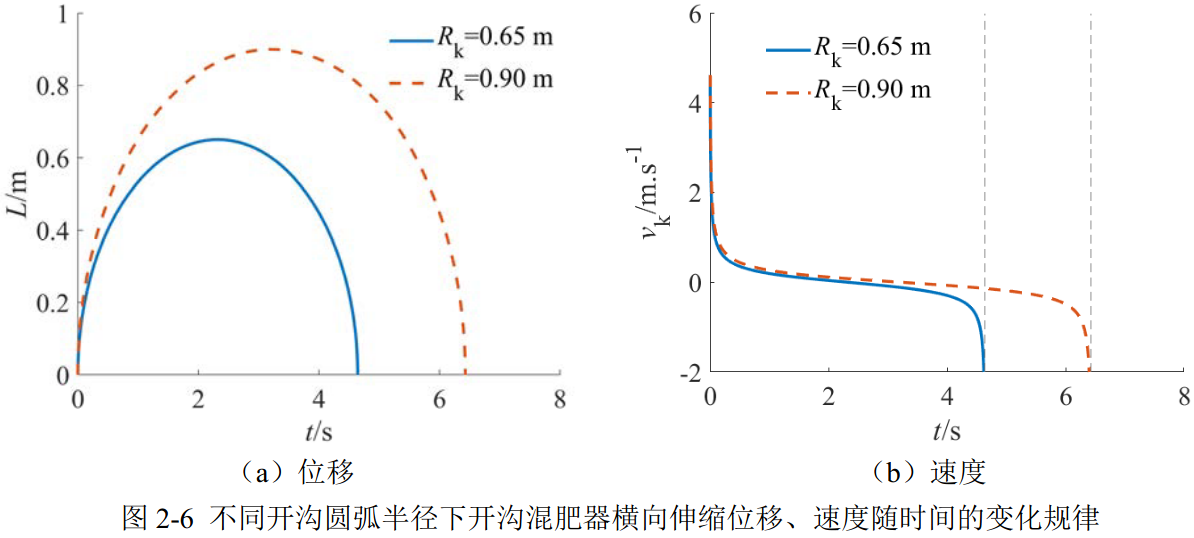
\includegraphics[width=\textwidth]{../assets/不同开沟圆弧半径下开沟混肥器横向伸缩位移、速度随时间的变化规律.png}
		
			\kaishu\raggedleft\href{https://doi.org/10.27409/d.cnki.gxbnu.2022.002616}{——果园机械化环沟施肥轨迹分析及控制系统研究 Page.27}
	\end{tcolorbox}

	
	该图像的坐标轴标签使用“/”分割变量符号和单位，存在歧义，容易被误认为是变量表达式，应该修改为“变量名(单位)”，并且变量名应使用倾斜字体，单位应使用直立字体。

	\section{想法}

	\subsection{开沟施肥器位置的控制机构}

	\begin{figure}[H]
		\centering
		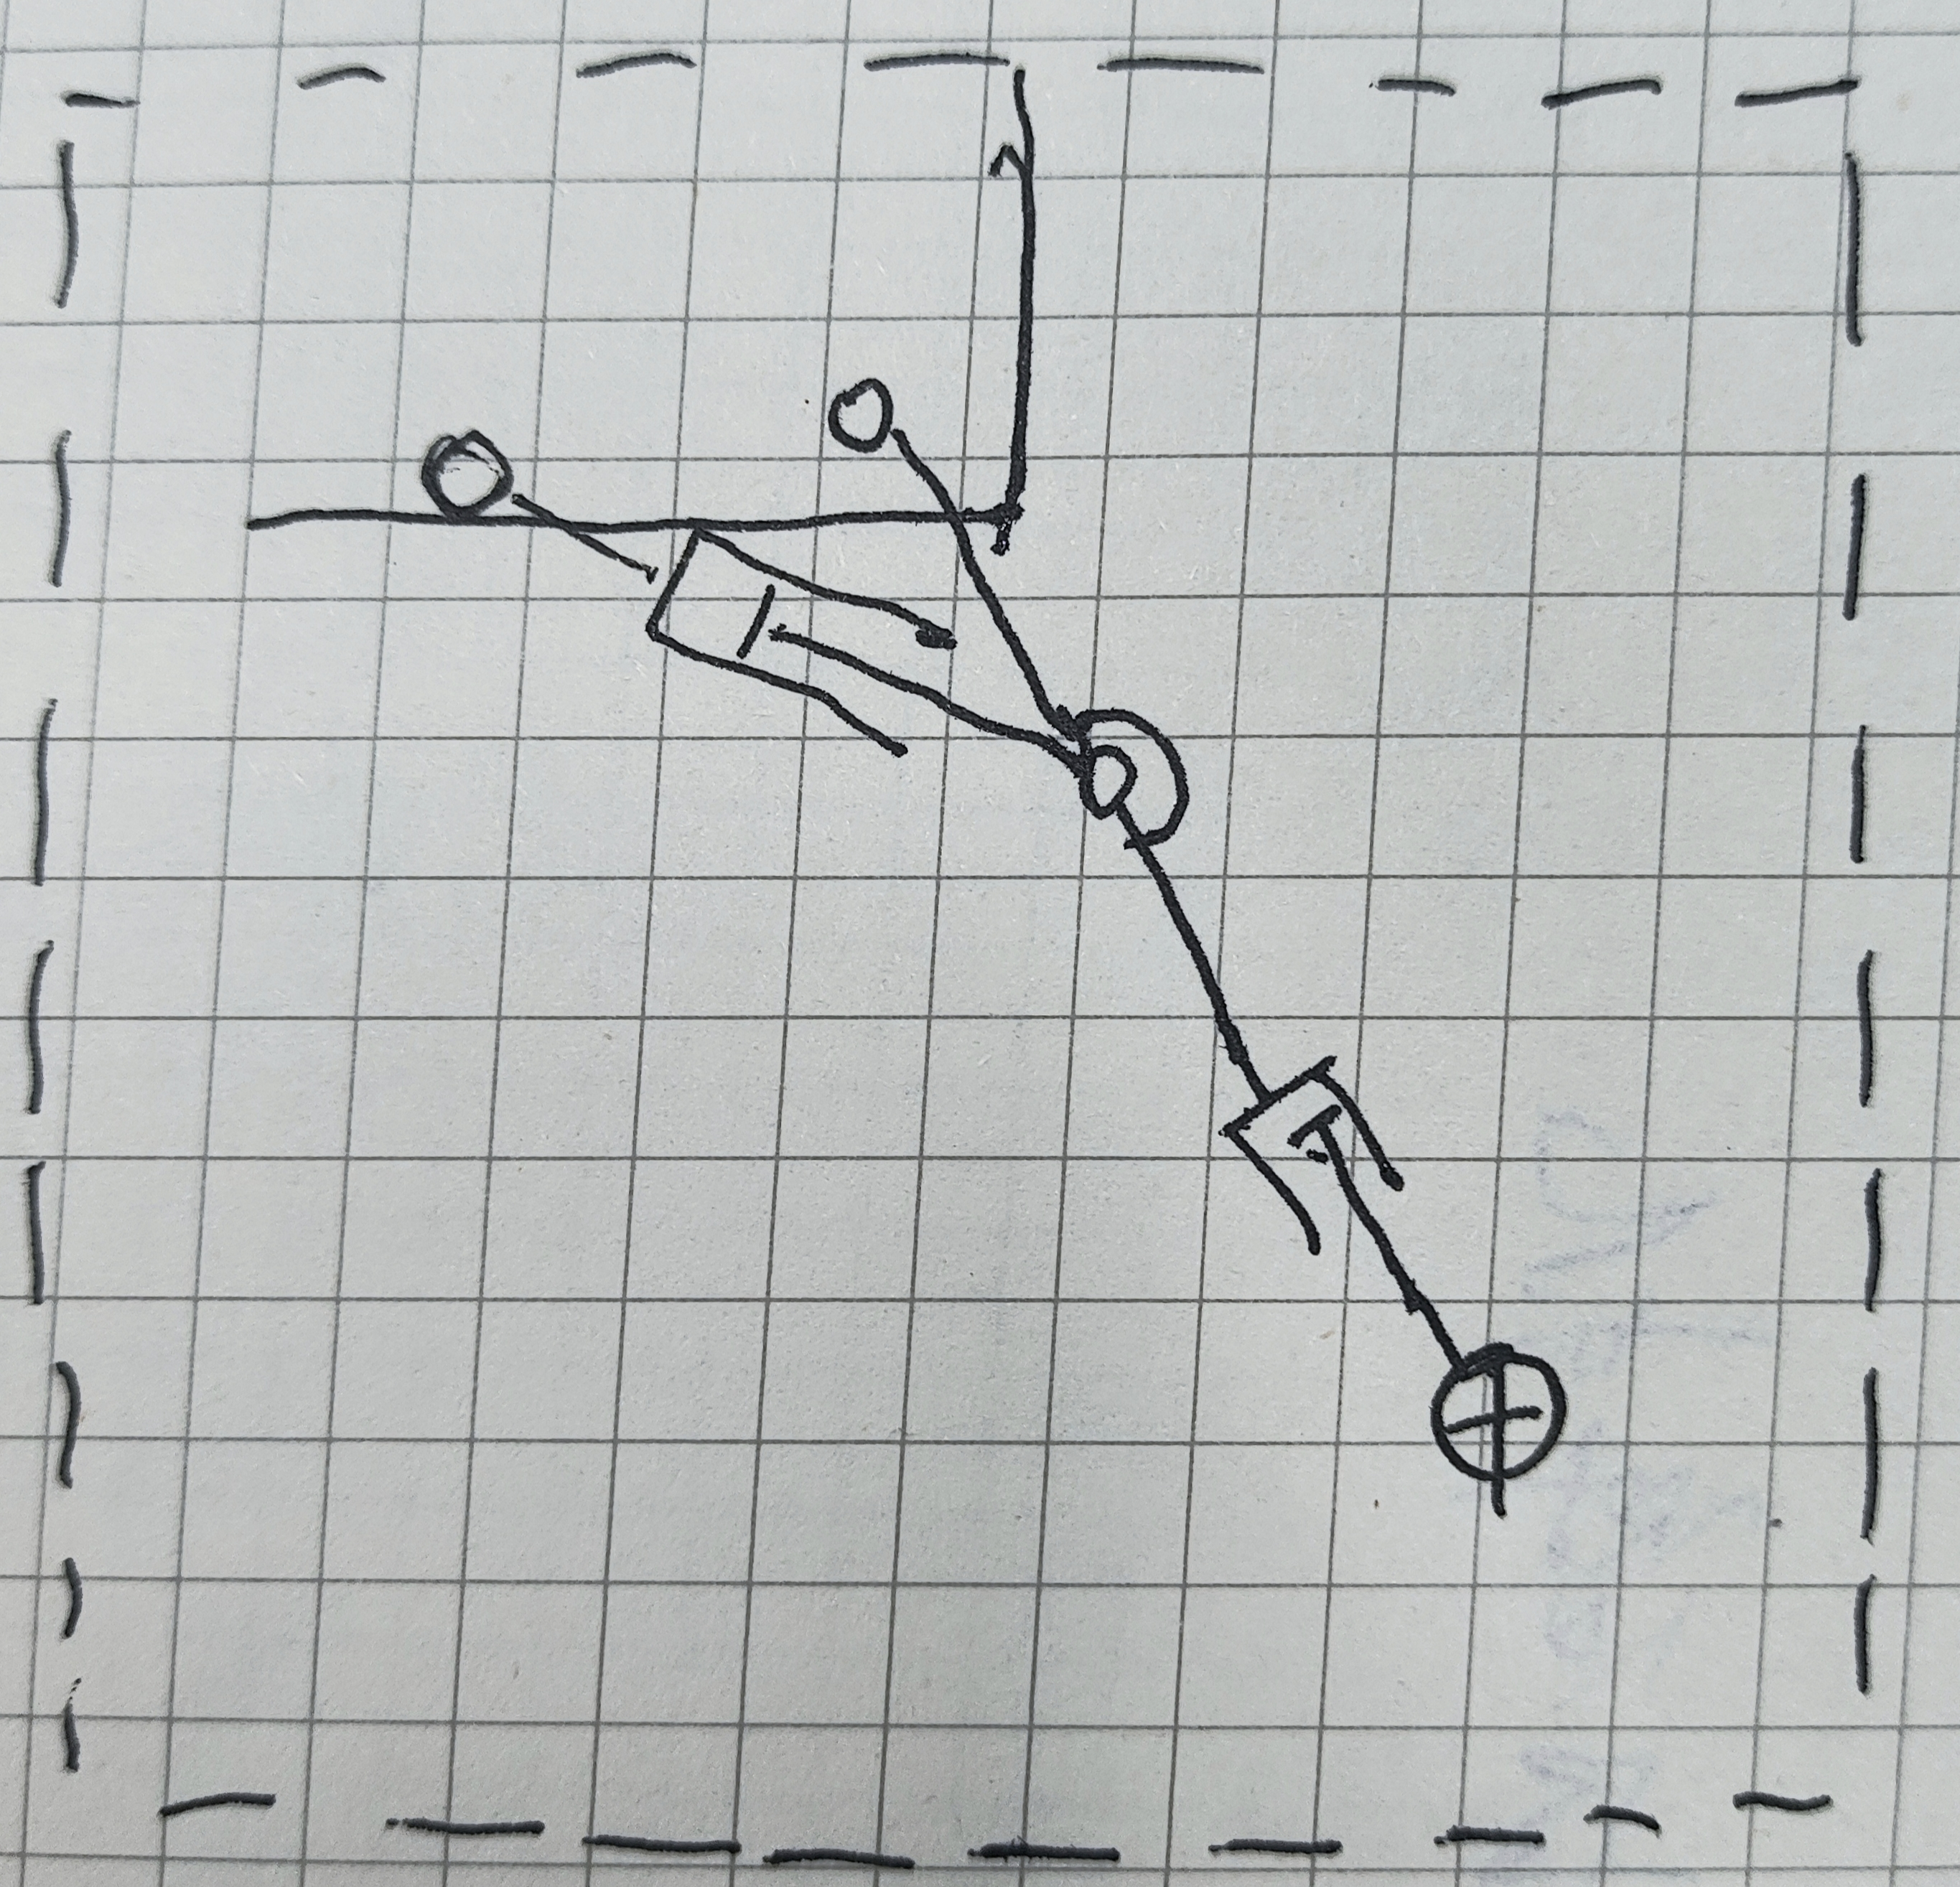
\includegraphics[width=0.8\textwidth]{../assets/曲线开沟施肥器位置控制结构想法.jpg}
		\caption{曲线开沟施肥器位置控制结构想法}
	\end{figure}
		
\end{document}